\documentclass{standalone}

\usepackage{tikz}

\usetikzlibrary{calc}

\begin{document}
  %noformat{
  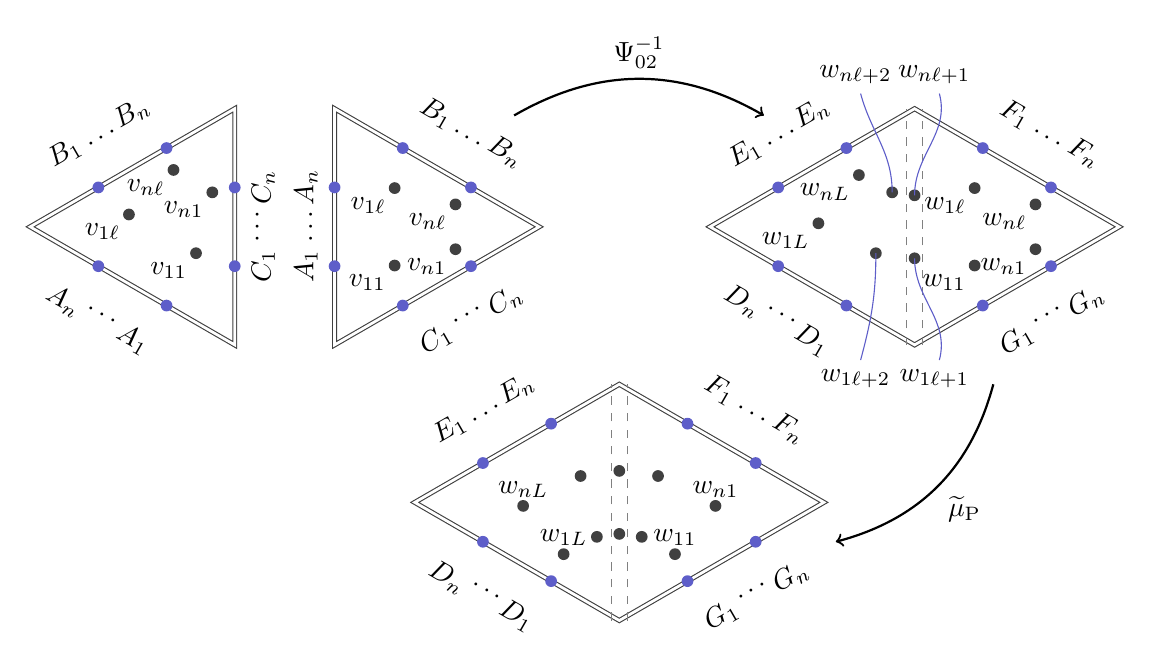
\begin{tikzpicture}
    \tikzstyle{v1} = [circle, outer sep=0.5pt, fill, inner sep=1.5pt]
    \tikzstyle{unf} = [color=darkgray]
    \tikzstyle{frz} = [color=blue!60!darkgray!70]
    \tikzstyle{e} = [->, >={stealth}]
    \tikzstyle{b} = [fill, fill opacity=0.0, circle, outer sep=0.5pt, inner sep=1.5pt]
    \tikzstyle{te} = [color=darkgray, double distance=1pt]
    \tikzstyle{h} = [dashed, color=gray, ->, >={stealth}]
    \tikzstyle{ll} = [color=blue!60!darkgray!70]

    \begin{scope}[shift={(0,0)}]
      \coordinate (l_0) at (-60:1.7321);
      \coordinate (l_1) at (180:1.7321);
      \coordinate (l_2) at ( 60:1.7321);

      \draw[te] (l_0) -- (l_1) -- (l_2) -- cycle;

      \node[v1, frz, label={240:{\rotatebox{330}{$A_1$}}}   ] at ($ (l_0) + (150:1.0) $) {};
      \node[b,       label={240:{\rotatebox{330}{$\cdots$}}}] at ($ (l_0) + (150:1.5) $) {};
      \node[v1, frz, label={240:{\rotatebox{330}{$A_n$}}}   ] at ($ (l_0) + (150:2.0) $) {};

      % As of writing, rotatebox{90}{} will crash on at least one machine
      \node[v1, frz, label={  0:{\rotatebox{ 90.001}{$C_1$}}}   ] at ($ (l_0) + ( 90:1.0) $) {};
      \node[b,       label={  0:{\rotatebox{ 90.001}{$\cdots$}}}] at ($ (l_0) + ( 90:1.5) $) {};
      \node[v1, frz, label={  0:{\rotatebox{ 90.001}{$C_n$}}}   ] at ($ (l_0) + ( 90:2.0) $) {};

      \node[v1, frz, label={120:{\rotatebox{ 30}{$B_1$}}}   ] at ($ (l_1) + ( 30:1.0) $) {};
      \node[b,       label={120:{\rotatebox{ 30}{$\cdots$}}}] at ($ (l_1) + ( 30:1.5) $) {};
      \node[v1, frz, label={120:{\rotatebox{ 30}{$B_n$}}}   ] at ($ (l_1) + ( 30:2.0) $) {};

      \node[v1, unf, label={[label distance=-3pt]210:$v_{1 \ell}$}] at ($ (l_2) + (225:1.9)$) {};
      \node[v1, unf, label={[label distance=-3pt]210:$v_{n \ell}$}] at ($ (l_2) + (225:1.1)$) {};
      \node[v1, unf, label={[label distance=-3pt]210:$v_{1 1}$}   ] at ($ (l_2) + (255:1.9)$) {};
      \node[v1, unf, label={[label distance=-3pt]210:$v_{n 1}$}   ] at ($ (l_2) + (255:1.1)$) {};
    \end{scope}

    \begin{scope}[shift={(3,0)}]
      \coordinate (r_0) at (240:1.7321);
      \coordinate (r_1) at (120:1.7321);
      \coordinate (r_2) at (  0:1.7321);

      \draw[te] (r_0) -- (r_1) -- (r_2) -- cycle;

      \node[v1, frz, label={180:{\rotatebox{ 90.001}{$A_1$}}}   ] at ($ (r_0) + ( 90:1.0) $) {};
      \node[b,       label={180:{\rotatebox{ 90.001}{$\cdots$}}}] at ($ (r_0) + ( 90:1.5) $) {};
      \node[v1, frz, label={180:{\rotatebox{ 90.001}{$A_n$}}}   ] at ($ (r_0) + ( 90:2.0) $) {};

      \node[v1, frz, label={-60:{\rotatebox{ 30}{$C_1$}}}   ] at ($ (r_0) + ( 30:1.0) $) {};
      \node[b,       label={-60:{\rotatebox{ 30}{$\cdots$}}}] at ($ (r_0) + ( 30:1.5) $) {};
      \node[v1, frz, label={-60:{\rotatebox{ 30}{$C_n$}}}   ] at ($ (r_0) + ( 30:2.0) $) {};

      \node[v1, frz, label={ 60:{\rotatebox{-30}{$B_1$}}}   ] at ($ (r_1) + (-30:1.0) $) {};
      \node[b,       label={ 60:{\rotatebox{-30}{$\cdots$}}}] at ($ (r_1) + (-30:1.5) $) {};
      \node[v1, frz, label={ 60:{\rotatebox{-30}{$B_n$}}}   ] at ($ (r_1) + (-30:2.0) $) {};

      \node[v1, unf, label={[label distance=-3pt]210:$v_{1 1}$}   ] at ($ (r_2) + (195:1.9)$) {};
      \node[v1, unf, label={[label distance=-3pt]210:$v_{n 1}$}   ] at ($ (r_2) + (195:1.1)$) {};
      \node[v1, unf, label={[label distance=-3pt]210:$v_{1 \ell}$}] at ($ (r_2) + (165:1.9)$) {};
      \node[v1, unf, label={[label distance=-3pt]210:$v_{n \ell}$}] at ($ (r_2) + (165:1.1)$) {};
    \end{scope}

    \begin{scope}[shift={(9.5,0)}]
      \coordinate (q_0) at (270:1.5);
      \coordinate (q_1) at (180:2.598);
      \coordinate (q_2) at ( 90:1.5);
      \coordinate (q_3) at (  0:2.598);

      \draw[te] (q_0) -- (q_1) -- (q_2) -- (q_3) -- cycle;

      \node[v1, frz, label={240:{\rotatebox{330}{$D_1$}}}   ] at ($ (q_0) + (150:1.0) $) {};
      \node[b,       label={240:{\rotatebox{330}{$\cdots$}}}] at ($ (q_0) + (150:1.5) $) {};
      \node[v1, frz, label={240:{\rotatebox{330}{$D_n$}}}   ] at ($ (q_0) + (150:2.0) $) {};

      \node[v1, frz, label={120:{\rotatebox{ 30}{$E_1$}}}   ] at ($ (q_1) + ( 30:1.0) $) {};
      \node[b,       label={120:{\rotatebox{ 30}{$\cdots$}}}] at ($ (q_1) + ( 30:1.5) $) {};
      \node[v1, frz, label={120:{\rotatebox{ 30}{$E_n$}}}   ] at ($ (q_1) + ( 30:2.0) $) {};

      \node[v1, frz, label={ 60:{\rotatebox{-30}{$F_1$}}}   ] at ($ (q_2) + (-30:1.0) $) {};
      \node[b,       label={ 60:{\rotatebox{-30}{$\cdots$}}}] at ($ (q_2) + (-30:1.5) $) {};
      \node[v1, frz, label={ 60:{\rotatebox{-30}{$F_n$}}}   ] at ($ (q_2) + (-30:2.0) $) {};

      \node[v1, frz, label={-60:{\rotatebox{ 30}{$G_1$}}}   ] at ($ (q_0) + ( 30:1.0) $) {};
      \node[b,       label={-60:{\rotatebox{ 30}{$\cdots$}}}] at ($ (q_0) + ( 30:1.5) $) {};
      \node[v1, frz, label={-60:{\rotatebox{ 30}{$G_n$}}}   ] at ($ (q_0) + ( 30:2.0) $) {};

      \node[v1, unf, label={[label distance=-3pt]225:$w_{1L}$}] at ($ (q_2) + (230:1.9)$) {};
      \node[v1, unf, label={[label distance=-3pt]225:$w_{nL}$}] at ($ (q_2) + (230:1.1)$) {};
      \node[v1, unf                                           ] at ($ (q_2) + (255:1.9)$) {};
      \node[v1, unf                                           ] at ($ (q_2) + (255:1.1)$) {};
      \node[v1, unf                                           ] at ($ (q_0) + ( 90:1.9)$) {};
      \node[v1, unf                                           ] at ($ (q_0) + ( 90:1.1)$) {};
      \node[v1, unf, label={[label distance=-3pt]210:$w_{11}$}] at ($ (q_3) + (195:1.9)$) {};
      \node[v1, unf, label={[label distance=-3pt]210:$w_{n1}$}] at ($ (q_3) + (195:1.1)$) {};
      \node[v1, unf, label={[label distance=-3pt]210:$w_{1\ell}$}] at ($ (q_3) + (165:1.9)$) {};
      \node[v1, unf, label={[label distance=-3pt]210:$w_{n\ell}$}] at ($ (q_3) + (165:1.1)$) {};

      \draw[color=gray, dashed] ($ (q_0) + (  0:0.1) $) -- ($ (q_2) + (  0:0.1) $);
      \draw[color=gray, dashed] ($ (q_0) + (180:0.1) $) -- ($ (q_2) + (180:0.1) $);

      \node (wnlp1lab) at ($ (q_2) + ( 60:0.5) $) {$w_{n\ell + 1}$};
      \node (w1lp1lab) at ($ (q_0) + (-60:0.5) $) {$w_{1\ell + 1}$};
      \draw[ll] (wnlp1lab) to[out=285,in=90] ($ (q_0) + ( 90:1.9) $);
      \draw[ll] (w1lp1lab) to[out=75,in=270] ($ (q_0) + ( 90:1.1) $);

      \node (wnlp2lab) at ($ (q_2) + ( 60:0.5) + (180:1) $) {$w_{n\ell + 2}$};
      \node (w1lp2lab) at ($ (q_0) + (-60:0.5) + (180:1) $) {$w_{1\ell + 2}$};
      \draw[ll] (wnlp2lab) to[out=285,in=90] ($ (q_2) + (255:1.1) $);
      \draw[ll] (w1lp2lab) to[out=75,in=270] ($ (q_2) + (255:1.9) $);
    \end{scope}

    \draw[->, thick]
        ($ (3,0) + ( 45:2) $)
        to[bend left] node[midway, above] (t01) {$\Psi_{02}^{-1}$}
        ($ (9,0) + (135:2) $);

    \begin{scope}[shift={(5.75,-3.5)}]
      \coordinate (q_0) at (270:1.5);
      \coordinate (q_1) at (180:2.598);
      \coordinate (q_2) at ( 90:1.5);
      \coordinate (q_3) at (  0:2.598);

      \draw[te] (q_0) -- (q_1) -- (q_2) -- (q_3) -- cycle;

      \node[v1, frz, label={240:{\rotatebox{330}{$D_1$}}}   ] at ($ (q_0) + (150:1.0) $) {};
      \node[b,       label={240:{\rotatebox{330}{$\cdots$}}}] at ($ (q_0) + (150:1.5) $) {};
      \node[v1, frz, label={240:{\rotatebox{330}{$D_n$}}}   ] at ($ (q_0) + (150:2.0) $) {};

      \node[v1, frz, label={120:{\rotatebox{ 30}{$E_1$}}}   ] at ($ (q_1) + ( 30:1.0) $) {};
      \node[b,       label={120:{\rotatebox{ 30}{$\cdots$}}}] at ($ (q_1) + ( 30:1.5) $) {};
      \node[v1, frz, label={120:{\rotatebox{ 30}{$E_n$}}}   ] at ($ (q_1) + ( 30:2.0) $) {};

      \node[v1, frz, label={ 60:{\rotatebox{-30}{$F_1$}}}   ] at ($ (q_2) + (-30:1.0) $) {};
      \node[b,       label={ 60:{\rotatebox{-30}{$\cdots$}}}] at ($ (q_2) + (-30:1.5) $) {};
      \node[v1, frz, label={ 60:{\rotatebox{-30}{$F_n$}}}   ] at ($ (q_2) + (-30:2.0) $) {};

      \node[v1, frz, label={-60:{\rotatebox{ 30}{$G_1$}}}   ] at ($ (q_0) + ( 30:1.0) $) {};
      \node[b,       label={-60:{\rotatebox{ 30}{$\cdots$}}}] at ($ (q_0) + ( 30:1.5) $) {};
      \node[v1, frz, label={-60:{\rotatebox{ 30}{$G_n$}}}   ] at ($ (q_0) + ( 30:2.0) $) {};

      \node[v1, unf, label={[label distance=-3pt] 90:$w_{nL}$}] at ($ (q_0) + (130:1.9)$) {};
      \node[v1, unf, label={[label distance=-3pt] 90:$w_{1L}$}] at ($ (q_0) + (130:1.1)$) {};
      \node[v1, unf                                           ] at ($ (q_0) + (105:1.9)$) {};
      \node[v1, unf                                           ] at ($ (q_0) + (105:1.1)$) {};
      \node[v1, unf                                           ] at ($ (q_0) + ( 90:1.9)$) {};
      \node[v1, unf                                           ] at ($ (q_0) + ( 90:1.1)$) {};
      \node[v1, unf                                           ] at ($ (q_0) + ( 75:1.9)$) {};
      \node[v1, unf                                           ] at ($ (q_0) + ( 75:1.1)$) {};
      \node[v1, unf, label={[label distance=-3pt] 90:$w_{n1}$}] at ($ (q_0) + ( 50:1.9)$) {};
      \node[v1, unf, label={[label distance=-3pt] 90:$w_{11}$}] at ($ (q_0) + ( 50:1.1)$) {};

      \draw[color=gray, dashed] ($ (q_0) + (  0:0.1) $) -- ($ (q_2) + (  0:0.1) $);
      \draw[color=gray, dashed] ($ (q_0) + (180:0.1) $) -- ($ (q_2) + (180:0.1) $);
    \end{scope}

    \draw[->, thick]
        ($ (10.5,-2)$)
        to[bend left] node[midway, below right] (t02) {$\widetilde{\mu}_{\mathrm{P}}$}
        ($ ( 8.5,-4)$);


  \end{tikzpicture}
  %}noformat
\end{document}
